
\chapter{COHORT AND PERIOD DATA} 
\label{sec:third}
\section{Data description}

Our analysis are based on data from the Human Mortality Database (HMD, Last modified: 26 Sep 2017), which are freely accessible at http:// www.mortality.org. 
The HMD contains aggregate mortality statistics such as death counts, population estimates, exposure to risk estimates, life tables as well as some other statistics. 
Input data files for more than 35 countries, are accessible from each country page. In the HMD, every country is identified by a specific code.
For example "NOR" identifies the national population of Norway .
We used " Deaths by Lexis triangles " and " Exposure-to-risk by Lexis triangles " as describe later in connection with figures \ref{fig:lower-and-upper-triangle} and \ref{fig:lower-and-upper-triangle for cohort}.

At the time of writing, the following periods, age  and cohorts were available for Norway:
For the period data we have information for all periods, from the calendar year 1846 to the calendar year 2014 and the age varying between 0 and 110+.
For the cohort data we have information for all ages until the age of the cohort in 2014.(e.g for the cohort born in 1960 we have information up to the age of 54.)



\section{Construction of the Lexis diagram}
    
Any dynamics such as births and deaths involve change over calendar time, age, and/or cohort. Those dynamics can be visualized with the help of the Lexis diagram, named after the German statistician, economist, and social scientist Wilhelm Lexis (1837-1914). For a review of Lexis diagram, see e.g. \textcite{C06}.

The lexis diagram consist of a Cartesian coordinate system where the calendar time ("period") is depicted on the x-axis and age on the y-axis. Every demographic event can therefore be located based on the time and age.
However, the Lexis diagram can not be resume to a Cartesian diagram because of two characteristics (\cite{C01}):
        \begin{itemize}
            \item[-]The Lexis diagram has two axes but allows the use of three separate coordinates. \item[-]Moreover, on the Lexis diagram each individual under observation belong to a forced trajectory from which he can not escape, namely his 'Life line'. 
        \end{itemize}
The life line is a specificity of Lexis diagram and it is essential for defining cohort.
Generally events that are observed on a Lexis diagram can be classified according to three coordinates. For example death will have:
        \begin{itemize}
         \item[-]The date of death (time designated by T), 
         \item[-]The age of the person at the time of death (age designated by A), 
         \item[-]and the moment of birth of the person (designated by M).
        \end{itemize}



%\newpage

        \begin{figure}[tbh]
         \centering
          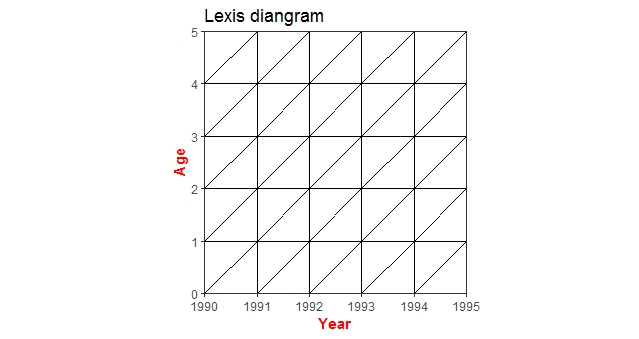
\includegraphics[width=\linewidth]{figures/lexis_plot1.jpeg}
          \caption{Lexis grid}
          \label{fig:lexis1}
        \end{figure}

On the  Figure~\ref{fig:lexis1} we have a lexis grid from year 1990 to year 1995, representing the age 0 to 5.
The units on those axes are identical. The moment of birth for each individual correspond to the age of exactly 0 year. The diagram is divided into 1 x 1 cells (i.e one year of age by one year of time). 
A simple mathematical relationship connects the three variables time, age and time of birth : A = T - M. Since these three variables are expressed in the same unit (year), all the life lines will have the same slope, drawing a 45 degrees angle with the time of birth axis.    
    
       
        \begin{figure}[tbh]
        \centering
        \begin{subfigure}{.5\textwidth}
          \centering
          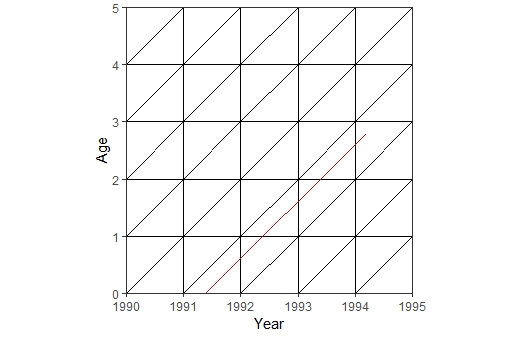
\includegraphics[width=1\linewidth]{figures/lexis_plot3.jpeg}
          \caption{}
          %\label{lexis 2}
        \end{subfigure}%
        \begin{subfigure}{.5\textwidth}
          \centering
          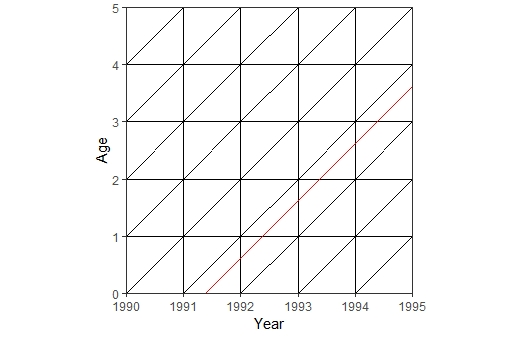
\includegraphics[width=1\linewidth]{figures/lexis_plot4.jpeg}
          \caption{}
          %\label{fig:lexis 2}
        \end{subfigure}
        \caption{Lexis diagram with life line}
        \label{fig:lexis 2}
        \end{figure}

Figure~\ref{fig:lexis 2} is a Lexis diagram  with the straight red lines representing  "life line". As we can observe, the line begins on the time axis at the person's birth. The line is continuous and the ends point represent the person's death. So in the figure on the left we have a person born the 23 of September 1991 and died on the 11 of June 1994. On the right we have the representation of a person born the 23th of September 1991 and still alive at the end of 1994. If we add together all the life line lengths in a particular portion of the Lexis diagram, we will obtain the person-years lived or exposure in that area. %During demography analysis, life lines are consider for both period and cohort data.   
   
     \begin{figure}[tbh]
         \centering
          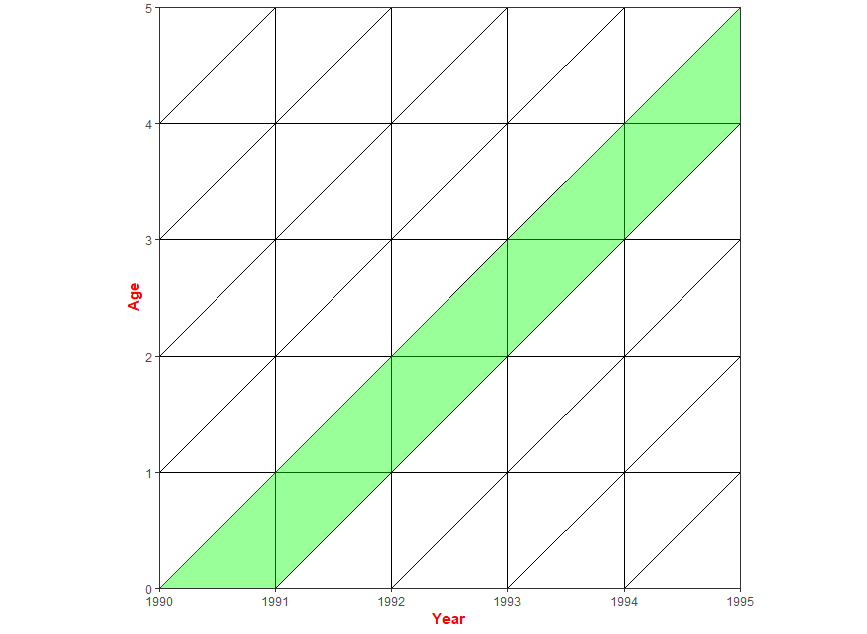
\includegraphics[scale=0.4]{figures/lexis_cohort.png}
          \caption{Cohort from 1990}
          \label{fig:lexis 3}
        \end{figure}  
   

A cohort can be defined as a group of persons who experience an event at the same time. On Figure~\ref{fig:lexis 3} we have a Lexis diagram presenting a cohort of persons born in the year 1990 and lived until the end of 1994. The Lexis diagram can present a cohort through their life experience or a cohort in a specific interval.    
    
     \begin{figure}[tbh]
         \centering
          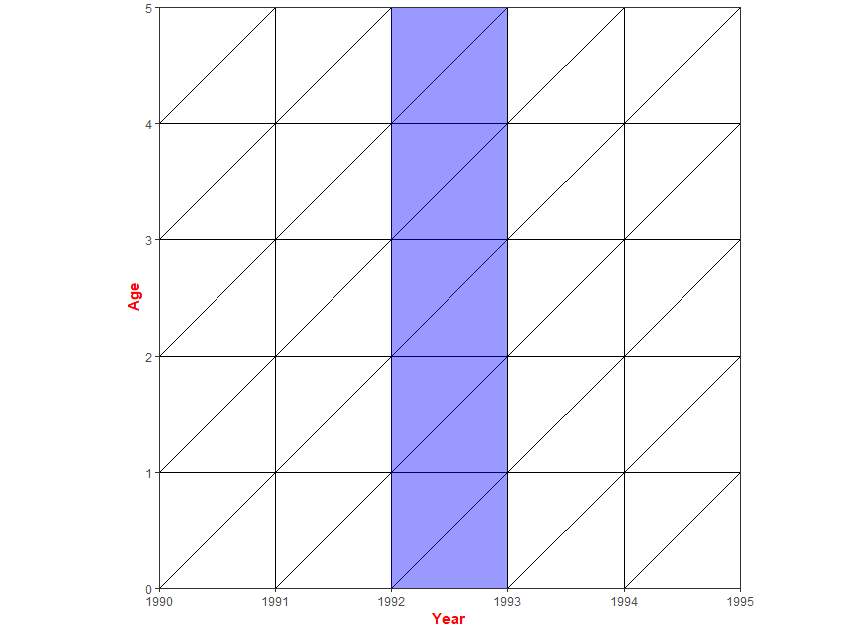
\includegraphics[scale=0.4]{figures/lexis_year.png}
          \caption{Lexis diagram with year 1992}
          \label{fig:lexis 4}
        \end{figure}
    
Many demographic investigations are conducted on period data. On Figure~\ref{fig:lexis 4} we have the age group from 0 year to 5 years during the year 1992, i.e population during year 1992. Finally, on Figure~\ref{fig:lexis 4} we have highlighted all points that belong to the age of 2 years.
     

             \begin{figure}[tbh]
         \centering
          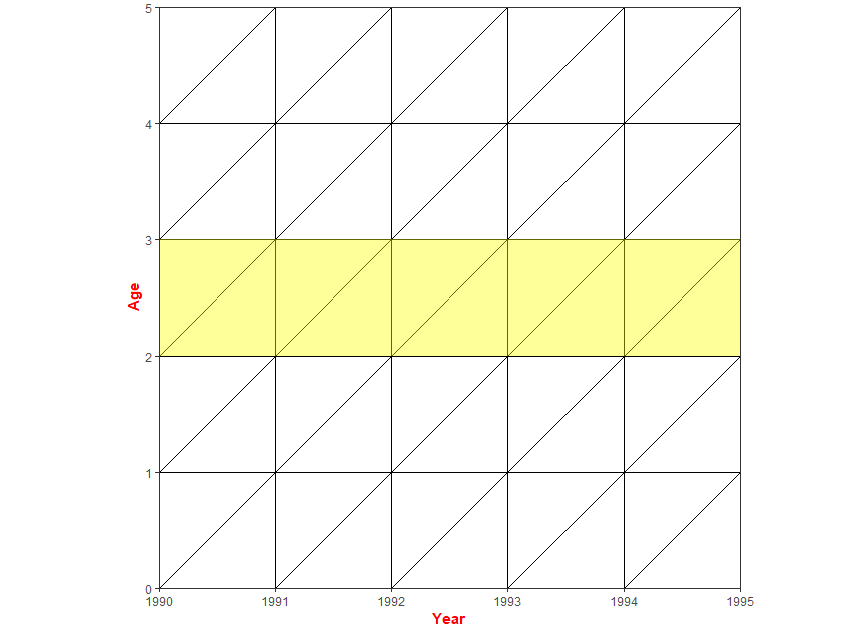
\includegraphics[scale=0.4]{figures/lexis_age.png}
          \caption{Lexis diagram with age group 2}
          \label{fig:lexis 5}
        \end{figure} 
     
   

    
        
         \begin{figure}[tbh]
         \centering
          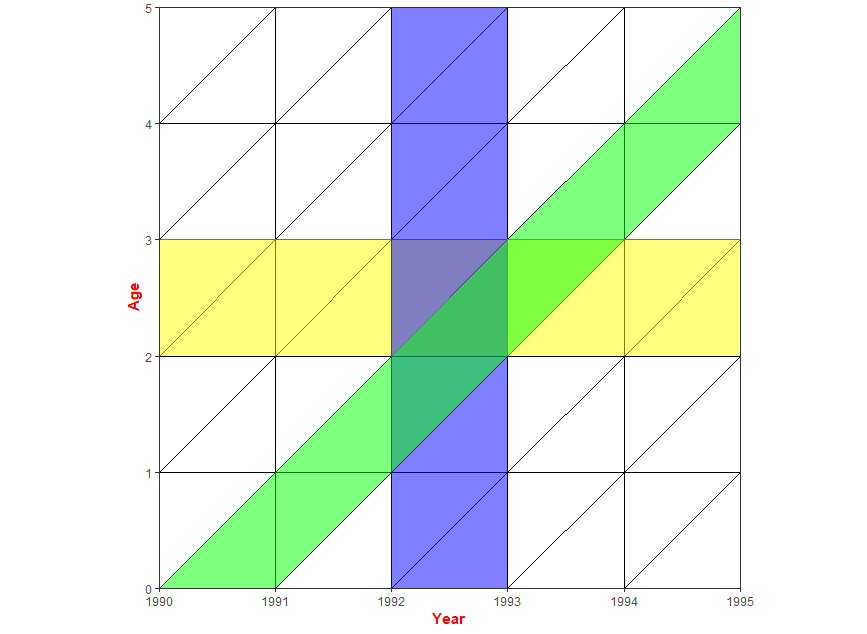
\includegraphics[scale=0.4]{figures/lexis_summary.png}
          \caption{Summary of Lexis with age, year and cohort}
          \label{fig:lexis 6}
        \end{figure}

        


%\parencite{AM69}
 
In summary, demographers use the term "diagram" to refer to their graphical representation of the data rather than "graph".
On the Lexis diagram, the x-axis and the y-axis usually support the calendar time and the age respectively. On this diagram it is possible to identify events according to two coordinates on the axes such as it is the case in any type of Cartesian diagram, but the Lexis diagram has the specificity of having a third coordinate, the moment of birth.
\parencite{Wal17}

 

\section{Mortality rate} 

One way of understanding population change is to measure and analyse its components. Demographers therefore measure events in terms of rates. 
A mortality rate $\hat{\mu}$ can be defined as the ratio of the number of deaths (D) in a specified time period by the exposure (i.e person-years) during the period (R): 

        \begin{equation}
          \hat{\mu} = \frac{D}{R}
          \label{mortality rate}
        \end{equation}
As shown previously in (\ref{Mu_hat}), this is the maximum likelihood estimate of the mortality hazard. 
We will first look at how the mortality rate is computed in the case of period data and then the cohort data.

\subsection{Period data}

An individual age $x$, where $x$ is an integer, has an exact age within the interval $[x, x+1)$. This concept is called "last birthday". 
Similarly an event that occurs in year t occurs during the calendar time interval $[t, t+1)$. 
The same apply to the exposure to risk of dying. The person-years age $x$ in year $t$ refers to all person-years lived in the age interval $[x, x+1)$ during calendar time $[t, t+1)$.
We assume that mortality hazard is constant over each one-year age interval and calendar year (period) and denote its value for age x and year t by ${\mu}_{x,t}$ see figure \ref{fig:mortality}.
The mortality hazard may be estimated by:

        \begin{equation}
          \hat{\mu}_{x,t}= 
          \frac{{D}_{x,t}}{{R}_{x,t}}
        \end{equation}
where ${D}_{x,t}$ is the number of deaths at age $x$ in year $t$ and ${R}_{x,t}$ the exposure (i.e person-years) at age $x$ in year $t$.  

If the coordinates of all life-lines are known, then the exposure  ${R}_{x,t}$ can be calculated precisely by adding up the length of each line segment within the cell. The actual length of each segment must be divided by $\sqrt{2}$, since life-lines are 45$^\circ$ from the age or time axes.
However in studies of large national populations we do not need to make calculations to obtain ${D}_{x,t}$ and ${R}_{x,t}$ because they may be obtained from the Human Mortality Database (HMD).
More specifically, what may be obtained from the HMD are the number of deaths and the exposures (i.e person years) for the triangles in lexis diagram.
We denote by ${D}_{x,t}^{(l)}$ and ${D}_{x,t}^{(u)}$ the number of deaths in the lower and upper triangles for age $x$ in year $t$, see figure \ref{fig:lower-and-upper-triangle}
and let ${R}_{x,t}^{(l)}$ and ${R}_{x,t}^{(u)}$ be the corresponding exposures.

    \begin{figure}[tbh]
    \begin{minipage}[b]{0.40\linewidth}
        \centering
        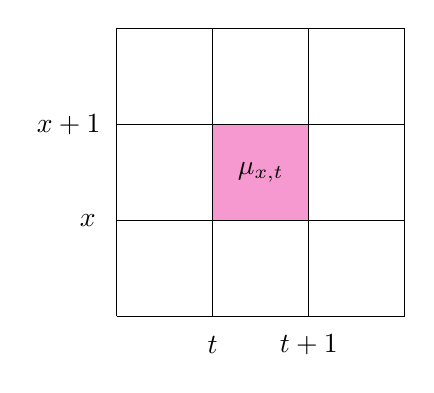
\begin{tikzpicture}[scale=1.22]
        \draw (0,0) grid (3,3);
        \draw (-0.3,1) node {$x$};
        \draw (-0.5,2) node {$x+1$};
        \draw (1,-0.3) node {$t$};
        \draw (2,-0.3) node {$t+1$};
        \filldraw[fill=magenta!40!white,] (1,1) rectangle (2,2);
        \draw (1.5,1.5) node {{${\mu}_{x,t}$}};
        \end{tikzpicture}
        \caption{ Mortality hazard for age x and year t.}
        \label{fig:mortality}
   \end{minipage}
  \hspace{0.5cm}
     \begin{minipage}[b]{0.40\linewidth}
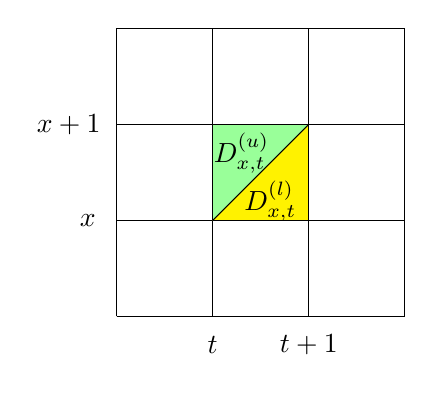
\begin{tikzpicture}[scale=1.22]
        \draw (0,0) grid (3,3);
        \draw (-0.3,1) node {$x$};
        \draw (-0.5,2) node {$x+1$};
        \draw (1,-0.3) node {$t$};
        \draw (2,-0.3) node {$t+1$};
       % \draw (3,-0.3) node {$t+2$};
        \filldraw[fill=green!40!white, draw=black] (1,1)-- (1,2)--(2,2);
        \filldraw[fill=yellow, draw=black] (1,1)-- (2,1)--(2,2);
        %\filldraw[fill=green, draw=black] (2,1)-- (2,2)--(3,2);
        \draw (1.6,1.2) node {$D_{x,t}^{(l)}$};
        \draw (1.3,1.7) node {$D_{x,t}^{(u)}$};
        %\draw (2.3,1.6) node {$D_{x,t+1}^{(u)}$};
        \draw (1,1) -- (2,2);
        %\draw (2,1) -- (3,2);
        \end{tikzpicture}
        \caption{ lower and upper triangle.  \label{fig:lower-and-upper-triangle}}
   \end{minipage}
   \end{figure}



In order to compute the mortality rate (\ref{mortality rate}) for the period data, we then add up the upper (blue) and the lower (yellow) Lexis triangle of the same cell. See figure \ref{fig:lower-and-upper-triangle}. This gives  
 
    \begin{equation}
        {D}_{x,t} = {D}_{x,t}^{(u)} + {D}_{x,t}^{(l)}
        \label{eq:death period}
    \end{equation}
and similar for the exposure:   
    \begin{equation}
        {R}_{x,t} = {R}_{x,t}^{(u)} + {R}_{x,t}^{(l)}
        \label{eq:exposure period}
    \end{equation}
    

\subsection{Cohort data}

For cohort data we assume constant mortality hazard in the parallelogram in figure \ref{fig:Mortality harzard for age x and Cohort c} and denote its value for cohort $c$ in age $x$ by ${\mu}_{x,c}$. 
In this case, we add together the deaths in the yellow and green triangles of figure \ref{fig:lower-and-upper-triangle for cohort} to obtain the number of deaths at age $x$ for the cohort born in year $c$.
The cohort death rates is then estimated by:
        \begin{equation}
          \hat{\mu}_{x,c}= \frac{{D}_{x,c}}{{R}_{x,c}}
        \end{equation}
where        
    \begin{equation}
            {D}_{x,c} = {D}_{x,c+x}^{(l)} + {D}_{x,c+x+1}^{(u)}
            \label{eq:death cohort}
    \end{equation} 
and similar for the exposure: 
      \begin{equation}
        {R}_{x,c} = {T}_{x,c+x}^{(l)} + {R}_{x,c+x+1}^{(u)}
        \label{eq:death cohort}
      \end{equation}  

      

   \begin{figure}[tbh]
      %\begin{minipage}[b]{0.40\linewidth}
        \centering
        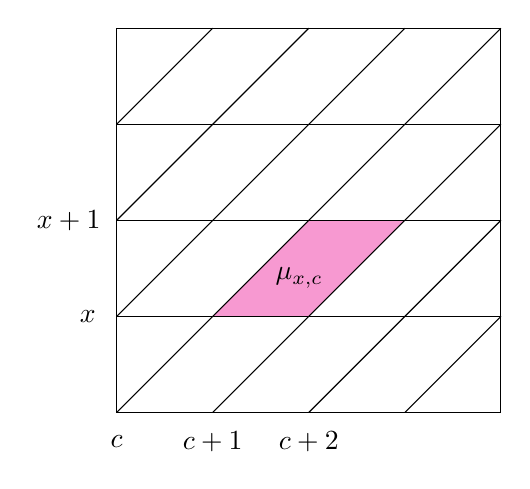
\begin{tikzpicture}[scale=1.22]
        \draw (0,0) rectangle (4,4);
        \draw (-0.3,1) node {$x$};
        \draw (-0.5,2) node {$x+1$};
        \draw (0,-0.3) node {$c$};
        \draw (1,-0.3) node {$c+1$};
        \draw (2,-0.3) node {$c+2$};
       \fill[fill=magenta!40!white,] (1,1)-- (2,1)--(2,2);
        \fill[fill=magenta!40!white,] (2,1)-- (2,2)--(3,2);
        %\draw (1.6,1.2) node {$D_{x,t}^{(l)}$};
        \draw (1.9,1.4) node {${\mu}_{x,c}$};
       % \draw (1,1) -- (2,2);
        %\draw (2,1) -- (3,2);
        \draw (0,0) -- (4,4);
        \draw (1,0) -- (4,3);
        \draw (2,0) -- (4,2);
        \draw (3,0) -- (4,1);
        \draw (0,1) -- (3,4);
        \draw (0,2) -- (2,4);
        \draw (0,3) -- (1,4);
        \draw (0,1) -- (4,1);
        \draw (0,2) -- (4,2);
        \draw (0,3) -- (4,3);
        \end{tikzpicture}
        \caption{ Mortality hazard for age x and Cohort c. \label{fig:Mortality harzard for age x and Cohort c}}
        %\end{minipage}
        
        \hspace{0.5cm}
        
       % \begin{minipage}[b]{0.40\linewidth}
        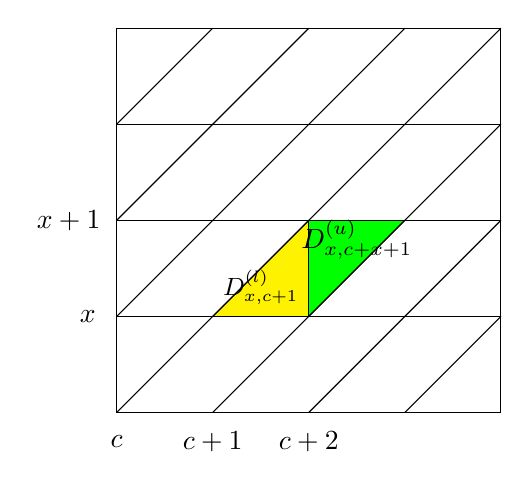
\begin{tikzpicture}[scale=1.22]
        \draw (0,0) rectangle (4,4);
        \draw (-0.3,1) node {$x$};
        \draw (-0.5,2) node {$x+1$};
        \draw (0,-0.3) node {$c$};
        \draw (1,-0.3) node {$c+1$};
        \draw (2,-0.3) node {$c+2$};
        \filldraw[fill=yellow!] (1,1)-- (2,1)--(2,2);
        \filldraw[fill=green!] (2,1)-- (2,2)--(3,2);
        \draw (1.5,1.3) node {{\small $D_{x,c+1}^{(l)}$}};
        \draw (2.5,1.8) node {$D_{x,c+x+1}^{(u)}$};
        \draw (1,1) -- (2,2);
        \draw (2,1) -- (3,2);
        \draw (0,0) -- (4,4);
        \draw (1,0) -- (4,3);
        \draw (2,0) -- (4,2);
        \draw (3,0) -- (4,1);
        \draw (0,1) -- (3,4);
        \draw (0,2) -- (2,4);
        \draw (0,3) -- (1,4);
        \draw (0,1) -- (4,1);
        \draw (0,2) -- (4,2);
        \draw (0,3) -- (4,3);
        \end{tikzpicture}
        \caption{ lower and upper triangle  \label{fig:lower-and-upper-triangle for cohort}}
        %\end{minipage}
       %\hspace{0.5cm}
   \end{figure}


 







\section{Plots of mortality rate}

         \begin{figure}[tbh]
             \centering
              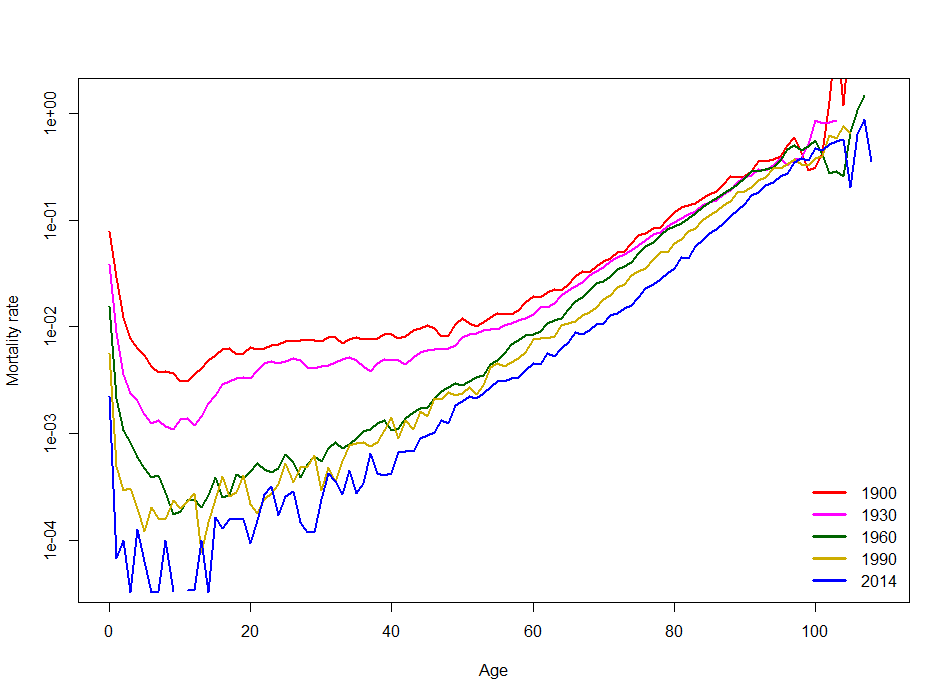
\includegraphics[width=0.8\linewidth]{figures/period_mortality_rate.png}
              \caption{Period mortality rate for Norwegian females.}
              \label{fig:period plot}
         \end{figure}



         
The graph in figure \ref{fig:period plot} presents the mortality rates for Norwegian females at each age for period data during the years 1900, 1930, 1960, 1990 and 2014.
The mortality rates are presented here on logarithmic scale "per 1000" person years. 
We can observe that the mortality rates are quite high just after birth and the first year of life. 
But the overall trend is that after this the rates of dying fall gradually, attaining minimum risk at age 5 for the year 2014 (graph in blue) and 15 for the year 1900 (graph in red). 
Then the risk starts increasing in adolescence, we can observed an exponential rise from one age year to the next.
From the age 100 and above, it may be difficult to have an accurate estimation because of the very low number of persons alive and therefore low number of deaths.

            \begin{figure}[tbh]
             \centering
              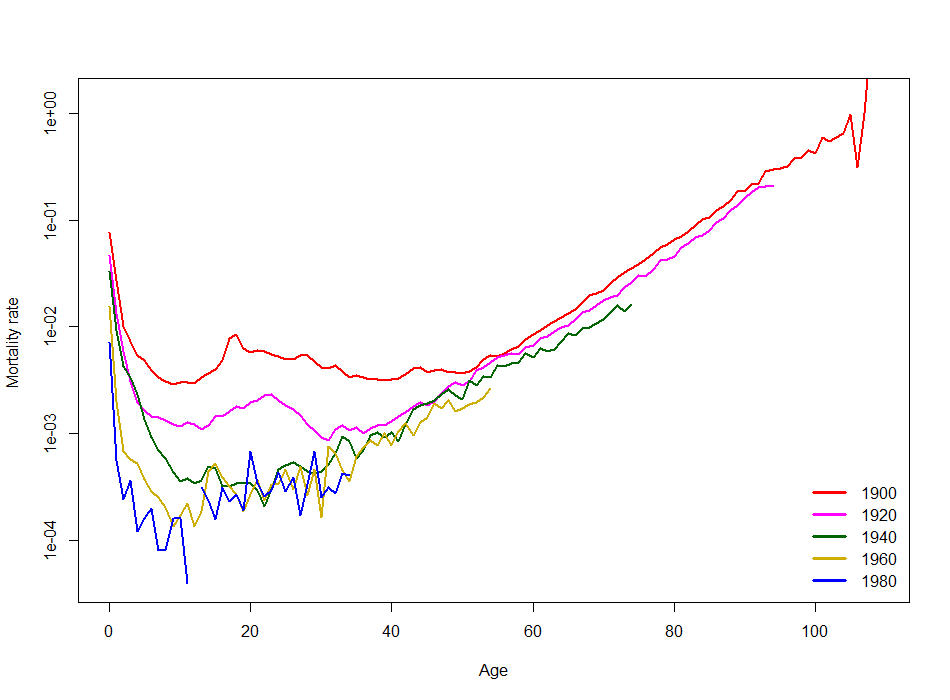
\includegraphics[width=0.8\linewidth]{cohort_mortality_rate.png}
              \caption{Cohort mortality rate for Norwegian females.}
              \label{fig:cohort plot}
            \end{figure}

The graph in figure \ref{fig:cohort plot} presents the mortality rates for females at each age for cohort data for the cohorts born in 1900, 1920, 1940, 1960 and 1980 in Norway.
As for the period data, we can observe here that the risk of dying is quite high immediately after birth but falls considerably reaching a minimum risk around 10 year for the cohort 1980 (graph in blue) and 15 for the cohort 1900 (graph in red). 
Between the age 18 and 43 we can observe some small fluctuations without any significant increase or decrease of the risk of dying. 
Around age 50 we can observe an exponential rise from one year to the next of the risk of dying. 
We also observe that the cohorts 1960 (graph in gold) and 1980 (graph in blue) stop at ages 54 and 34 respectively. 
That is due to the fact that we don't have data after that age for these cohorts.
As seen in graphs in figures \ref{fig:period plot} and \ref{fig:cohort plot} we can conclude that there is a continuous decrease of the risk of dying from year to year for all age groups. This mortality decline could be a result of an improvement of healthy lifestyle and diet during the past years and the development of new drugs and techniques in the medical field.




            \begin{figure}[tbh]
             \centering
              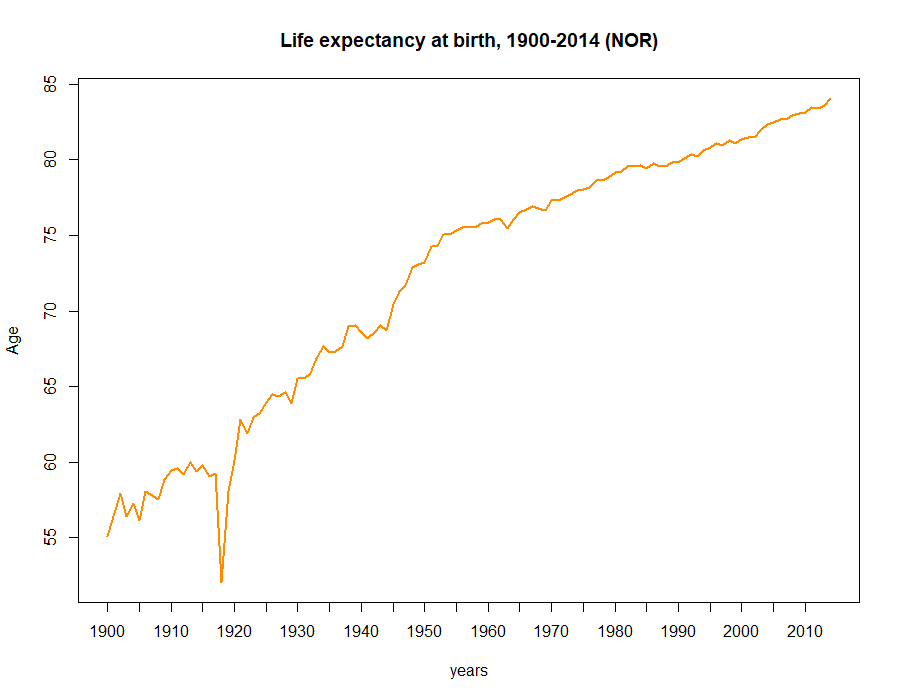
\includegraphics[width=0.8\linewidth]{period_life_expectancy.png}
              \caption{Life expectancy at birth for Norwegian females, period data.}
              \label{fig:period life expectancy}
            \end{figure}

\section{Life expectancy}


Life expectancy in any given year can be defined as the average number of years a person born in that year is expected to live if mortality rates at each age were to remain the same in the future. 
The life expectancy can be shown separately for males and females, as well as a combined figure. 
In figures \ref{fig:period life expectancy} and \ref{fig:cohort life expectancy} we focus on Norwegian females.
Life expectancy can be used as a measure or indicator of the quality of healthcare in a country, an ongoing war, or a pandemic.
Figure \ref{fig:period life expectancy} shows the evolution of the life expectancy at birth for Norwegian females in the period 1900-2014.
In 1900, life expectancy was 55.09 years and 84.09 years for 2014.
We observe that life expectancy has increased more or less continuously over the years, but  in 1918 we can see a clear interruption due to the Spanish flu pandemic. 
It went from 59.05 years two years earlier (1916) to 52.03 years in 1918, that is a loss of about 7 years in life expectancy in a very short period of time.
We also observe a little fluctuation from year to year during the period 1900-1916 and a small decrease during the world wars.



            \begin{figure}[tbh]
             \centering
              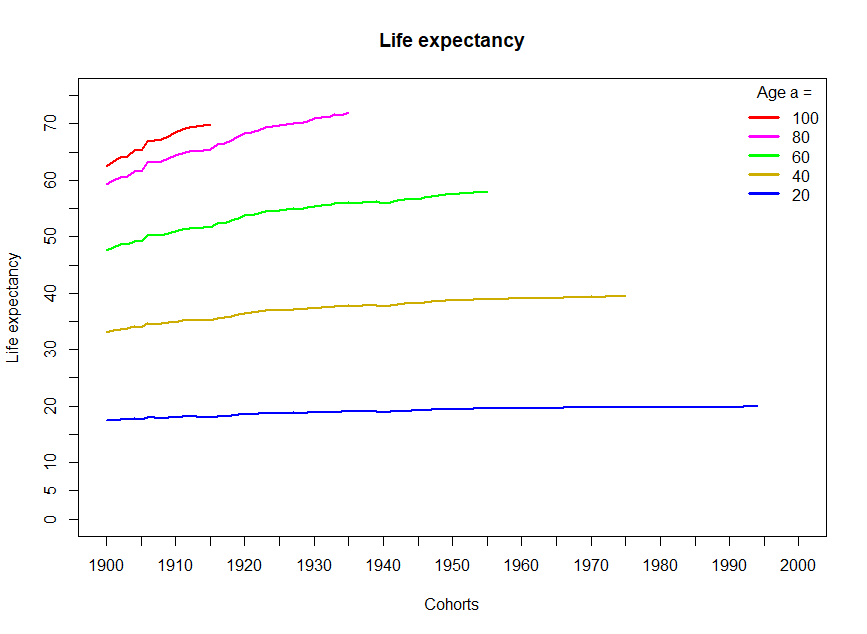
\includegraphics[width=0.8\linewidth]{figures/life_expectancy_cohort.png}
              \caption{Life expectancy up to age \textit{a} as a function of cohort for different choices of \textit{a} for Norwegian females.}
              \label{fig:cohort life expectancy}
            \end{figure}




Figure \ref{fig:cohort life expectancy} shows the life expectancy up to a certain age \textit{a} for different choices of \textit{a} for cohorts of Norwegian females. 
In this case we fix the age \textit{a} and consider life expectancy as a function of the cohort \textit{c}.
The cohorts vary between 1900 and 2010.
The life expectancy up to 100 years for the cohort born in 1900 was 62.43 years and 69.93 years for the cohort born in 1915.
That is an increase of 7.05 years. 
The evolution for that age group can be observed on the plot in red. 
The life expectancy up to 80 years for the cohort born in 1920 was 68.35 years and 71.97 years for the cohort born in 1935. Between 1920 and 1935 we observe an increase of 3.62 years (magenta line).
The increase of life expectancy for age 100 and 80 and their various cohorts is due to the drop in mortality we saw in figure \ref{fig:cohort plot}. 
For the age 60 and cohorts born in 1940, 1950 and 1955, we obtain respectively 55.95 years, 57.54 years and 57.94 years.
That can been observed on the green line. 
On the line in gold, with age 40 and cohorts 1960, 1970 and 1975, we obtain respectively 39,06 years, 39,36 years and 39,42 years. 
For the, age 20 and cohorts 1980, 1990 and 1995 we obtain respectively 19.82 years, 19.85 years and 19.90 years (blue line).
The life expectancy up the ages 60, 40 and 20 and their various cohorts have a small increase. Most of the individual in those different cohorts are still alive while the individuals for the cohort 1900, 1920 and 1935 are all death or almost all death.
%https://www.cairn.info/revue-sante-publique-2001-2-page-137.htm#

100 years is the maximum age, that means we will need 100 years of data for each cohort between 1900 and 2010. But that is not possible since very few cohorts have 100 years of data. To avoid this problem we have above used the "partial" life expectancy, that i.e we take the number of years lived up to a certain age \textit{a} (e.g. 100, 80, 60, 40, 20 …).

            
            \begin{figure}[tbh]
             \centering
              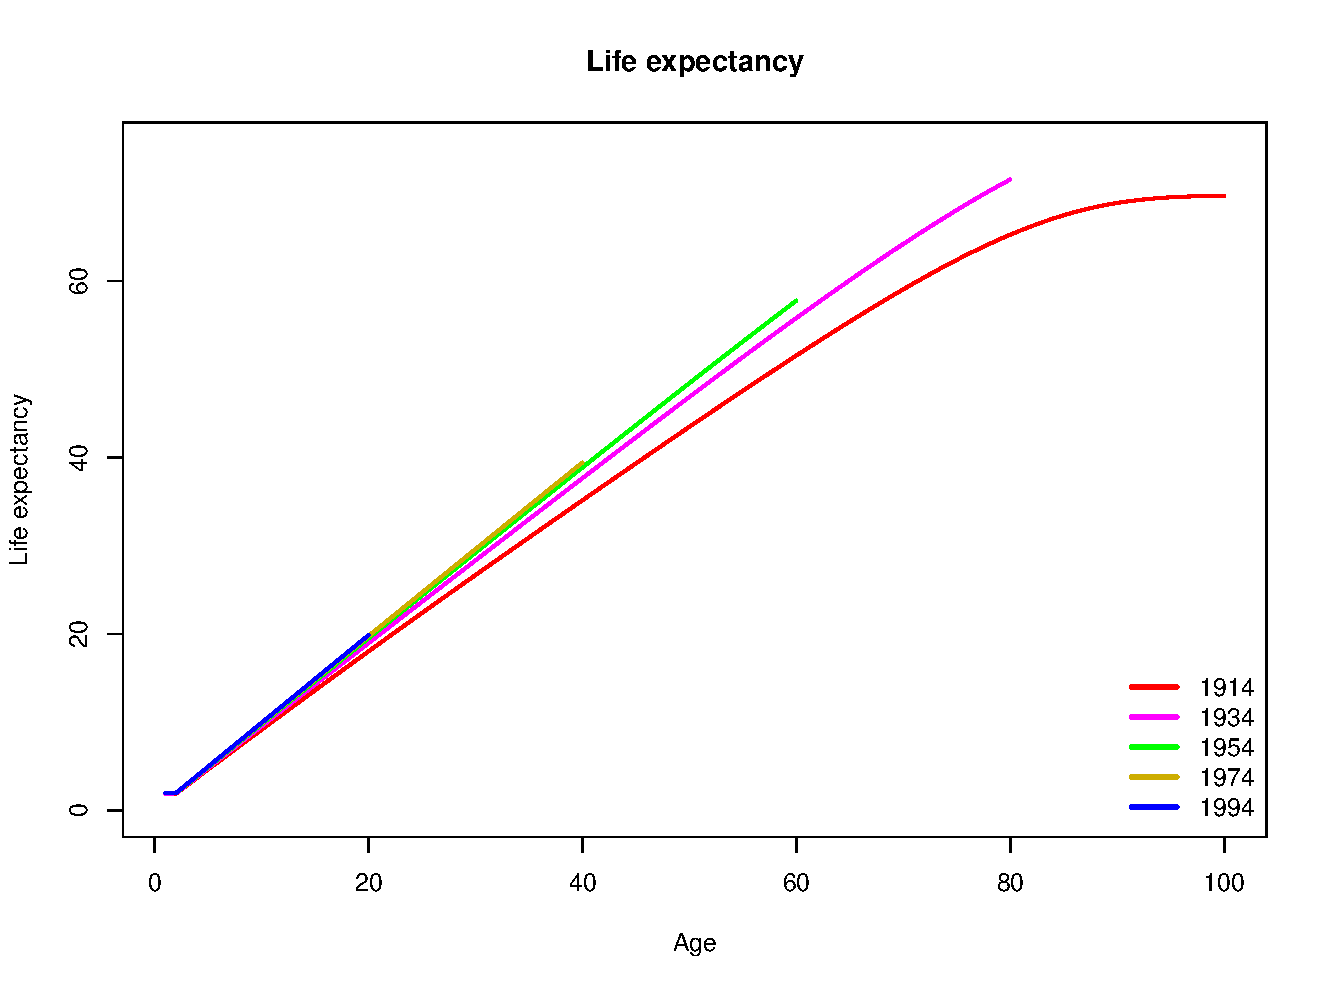
\includegraphics[ width=0.8\linewidth]{figures/cohortLife_expect_as_a_functionOf_Age.pdf}
              \caption{Life expectancy up to age \textit{a} as a function of \textit{a} for different cohorts of Norwegian females.}
              \label{fig:cohort as a function of age Norway}
            \end{figure}







            \begin{figure}[tbh]
             \centering
              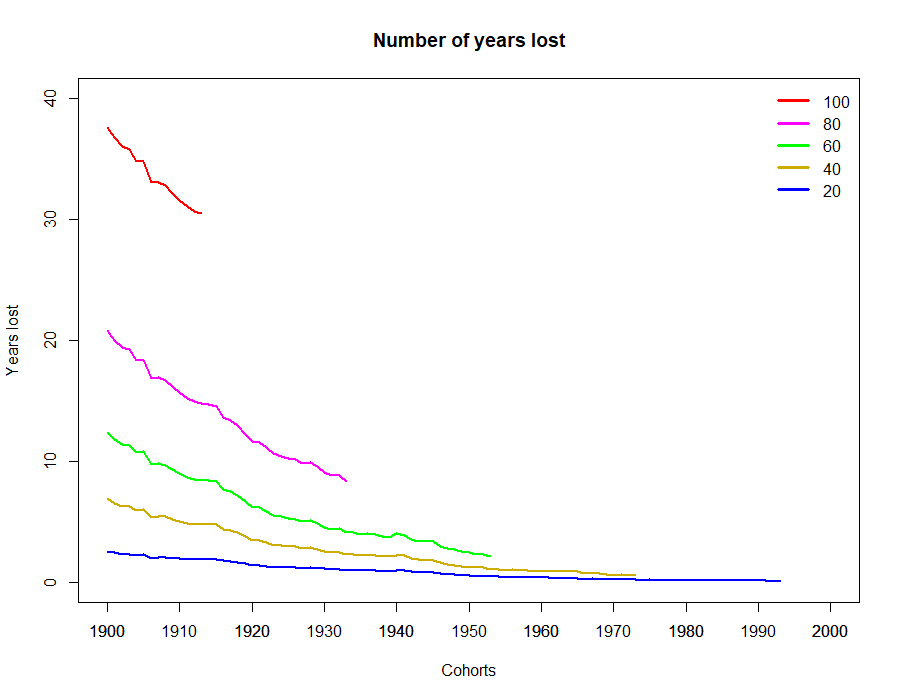
\includegraphics[ width=0.8\linewidth]{figures/yearLostAsFunctionOfCohort.png}
              \caption{Expected number of years lost up to age \textit{a} as a function of cohort for different choices of \textit{a} for Norwegian females.}
              \label{fig:number of years lost cohort}
            \end{figure}

If there had been no mortality, the partial life expectancy up to age \textit{a} would have been equal to \textit{a} years.
When there is mortality, the difference between age \textit{a} and the partial life expectancy up to age \textit{a} is called the expected number of years lost up to age \textit{a}:
 
 \begin{equation*}
 a - E[T_{a}]   
\end{equation*}

            
            
            
            \begin{figure}[tbh]
             \centering
              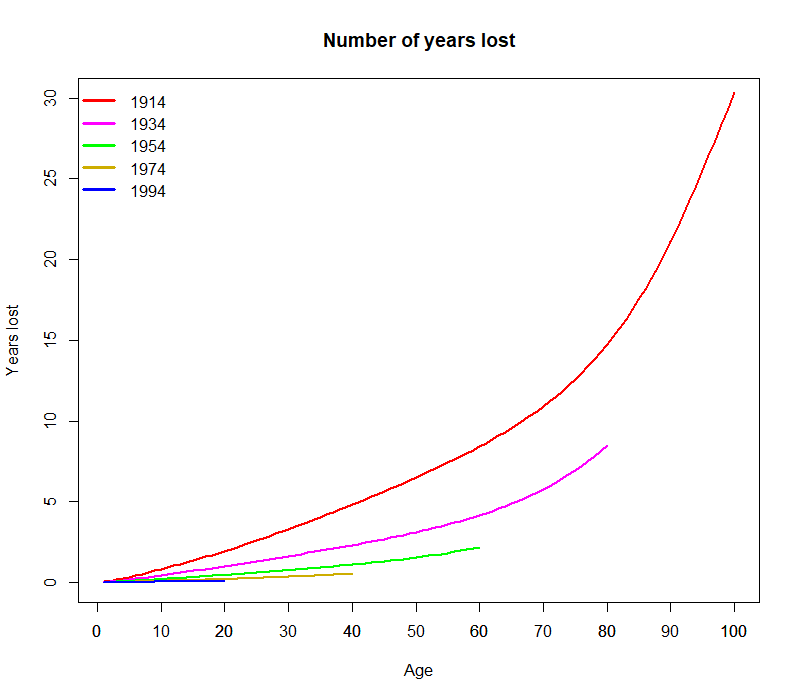
\includegraphics[ width=0.8\linewidth]{figures/yearLostAsFunctionOfAge.png}
              \caption{Expected number of years lost up to age \textit{a} as a function of \textit{a} for different cohorts of Norwegian females.}
              \label{fig:number of years lost age}
            \end{figure}
            
            
On the figures \ref{fig:number of years lost cohort} and \ref{fig:number of years lost age} we have the plots of the expected number of years lost up to age \textit{a}, first as a function of cohort for given age and then as a function of age for given cohorts for Norwegian women.
We can observe on the figures that for all ages the number of years lost is lower for the more recent cohorts than the earlier ones.
In the next chapter, we will apply the same methodology to some countries in Scandinavia and in the Mediterranean and compare the evolution of life expectancy in those two regions. 

            
            
          